\documentclass[conference]{IEEEtran}
\usepackage{natbib}
\usepackage{url}
\usepackage{hyperref}
\usepackage{framed}
\usepackage{mdframed}
\usepackage{tcolorbox}
\ifCLASSINFOpdf

\else

\fi

\hyphenation{op-tical net-works semi-conduc-tor}


\begin{document}

\title{\textbf{Roamify: Roaming Redefined}\\ \textit{Changing the Way World Travels}}


\author{\IEEEauthorblockN{Vikranth Udandarao}
\IEEEauthorblockA{Computer Science Engineering Dept\\
IIIT Delhi\\
Email: vikranth22570@iiitd.ac.in}
\and
\IEEEauthorblockN{Harsh Mistry}
\IEEEauthorblockA{Computer Science Engineering Dept\\
IIIT Delhi\\
Email: harsh22200@iiitd.ac.in}
\and
\IEEEauthorblockN{Muthuraj Vairamuthu}
\IEEEauthorblockA{Computer Science Engineering Dept\\
IIIT Delhi\\
Email: muthuraj22307@iiitd.ac.in}
\and
\IEEEauthorblockN{Noel Tiju}
\IEEEauthorblockA{Computer Science Engineering Dept\\
IIIT Delhi\\
Email: noel22338@iiitd.ac.in}
\and
\IEEEauthorblockN{Armaan Singh}
\IEEEauthorblockA{Computer Science Engineering Dept\\
IIIT Delhi\\
Email: armaan22096@iiitd.ac.in}
\and
\IEEEauthorblockN{Dhruv Kumar}
\IEEEauthorblockA{Computer Science Engineering Dept\\
IIIT Delhi\\
Email: dhruv.kumar@iiitd.ac.in}}



% \author{
%     \IEEEauthorblockN{Vikranth Udandarao} \vspace*{3.0pt}
%     \IEEEauthorblockA{
%         \textit{Computer Science \& Engineering Dept.} \\
%         \textit{IIIT-Delhi, India} \\
%         vikranth22570@iiitd.ac.in
%     }
%     \and
%     \IEEEauthorblockN{Harsh Mistry} \vspace*{3.0pt}
%     \IEEEauthorblockA{
%         \textit{Computer Science \& Engineering Dept.} \\
%         \textit{IIIT-Delhi, India} \\
%         harsh22200@iiitd.ac.in
%     }
%     \IEEEauthorblockN{Muthuraj Vairamuthu} \vspace*{3.0pt}
%     \IEEEauthorblockA{
%         \textit{Computer Science \& Engineering Dept.} \\
%         \textit{IIIT-Delhi, India} \\
%         muthuraj22...@iiitd.ac.in
%     }
%     \and
%     \IEEEauthorblockN{Noel Tiju} \vspace*{3.0pt}
%     \IEEEauthorblockA{
%         \textit{Computer Science \& Engineering Dept.} \\
%         \textit{IIIT-Delhi, India} \\
%         noel22338@iiitd.ac.in
%     }
%     \and
%     \IEEEauthorblockN{Armaan Singh} \vspace*{3.0pt}
%     \IEEEauthorblockA{
%         \textit{Computer Science \& Engineering Dept.} \\
%         \textit{IIIT-Delhi, India} \\
%         armaan22096@iiitd.ac.in
%     }
% }



% \author{\IEEEauthorblockN{Vikranth Udandarao\IEEEauthorrefmark{1},
% Harsh Mistry\IEEEauthorrefmark{1},
% Muthuraj Vairamuthu\IEEEauthorrefmark{1},
% Noel Tiju\IEEEauthorrefmark{1},
% Armaan Singh\IEEEauthorrefmark{1}}
% \IEEEauthorblockA{\IEEEauthorrefmark{1}Computer Science Engineering Dept\\
% IIIT Delhi\\
% }}




\maketitle

\begin{abstract}

    Travel planning is often cumbersome. Roamify, an AI-driven itinerary service, aims to simplify this by providing curated suggestions based on user preferences. Leveraging advanced NLP models, Roamify generates personalized travel plans, enhancing the travel experience by transforming it from mere logistics to memorable adventures. This paper details Roamify's innovative approach, methodologies, and its potential to redefine travel planning.

\end{abstract}

\IEEEpeerreviewmaketitle

\section{Introduction}

    \textbf{Roamify} - Roaming Redefined is on a transformative mission to revolutionize travel planning for today's generation. Aimed at youngsters, teenagers, college students, and families seeking seamless travel experiences, Roamify addresses a common dilemma: the desire to explore without the hassle of planning. Drawing inspiration from personal experiences with itinerary complexities, Roamify emerges as an innovative solution, leveraging AI-generated itineraries to provide curated suggestions tailored to travelers' destination preferences. This introduction sets the stage for exploring how Roamify redefines roaming, making travel not just about reaching a destination but also about unlocking memorable experiences along the way.

    In the past, travel was a luxury limited to the rich and elite. However, with advancements in transportation, travel has become more accessible to everyone. People now travel for various reasons: work, leisure, relaxation, reunions with friends, or simply for the joy of exploring new places. This increase in travel purposes has led to a new challenge: deciding what to explore upon arrival.
    
    Imagine a family of four planning a vacation during the kids' summer holidays. In the past, their only option was to visit an offline travel agency to book a package that included all the itineraries and attractions. With technological advancements, numerous online platforms have emerged, allowing people to customize and choose their own itineraries.
    
    Despite these advancements, a significant problem persists: many online travel websites struggle to attract users, even after being in existence for several years. Additionally, while tools like ChatGPT offer some assistance, they have limitations, such as outdated training data.
    
    Roamify aims to address these issues by integrating seamlessly with users' web browsers. Recognizing that travelers often have multiple tabs open while planning their trips, Roamify leverages this browsing behavior to provide intelligent recommendations based on the websites and tabs users have open. For instance, if a user has a tab open on a site like MakeMyTrip, Roamify identifies the flight destination and redirects the user to a site relevant to that destination. It then uses NLP processing to decode the webpage into attractions and sends this data to Llama for detailed itinerary generation. This innovative approach ensures that travel planning becomes more efficient and personalized, making Roamify an essential tool for modern travelers.

    The development and fine-tuning of the models used in Roamify were meticulously documented and are available on our GitHub and Hugging Face respectively: \href{https://github.com/RoamifyRedefined/Machine-Learning}{\textbf{RoamifyRedefined/Machine-Learning}} \& \href{https://huggingface.co/Roamify}{\textbf{huggingface.co/Roamify}}.


\section{Literature Review}

    In recent years, advancements in natural language processing (NLP) have significantly enhanced the ability of machine learning models to understand and generate human language. These advancements have been particularly beneficial for applications requiring detailed textual analysis and generation, such as travel itinerary planning. This paper presents a comparative study of five state-of-the-art NLP models—BERT, T5, DistilBERT, Llama, and RoBERTa—fine-tuned to generate personalized travel itineraries. By leveraging these models, we aim to redefine the travel planning experience through Roamify, an AI-powered itinerary generation service.

    \subsection{BERT (Bidirectional Encoder Representations from Transformers)}
        BERT, developed by Google, is a transformer-based model designed to understand the context of a word in search queries. Its bidirectional approach allows it to consider both the left and right context of a word, making it highly effective for tasks such as question answering and language understanding. In this study, we fine-tuned BERT for the task of generating travel itineraries, leveraging its deep understanding of context to provide precise and relevant recommendations.

    \subsection{T5 (Text-To-Text Transfer Transformer)}
        T5, also developed by Google, is a versatile model that treats all NLP tasks as a text-to-text problem. This unified approach allows T5 to be applied to a wide range of tasks by simply converting them into text generation tasks. For Roamify, we fine-tuned T5 to generate detailed travel itineraries based on user preferences and historical travel data, capitalizing on its ability to generate coherent and contextually accurate text.

    \subsection{DistilBERT}
        DistilBERT is a smaller, faster, and more efficient version of BERT, retaining 97\% of its language understanding capabilities while being 60\% faster and 40\% smaller. This model was fine-tuned to perform similar tasks as BERT but with reduced computational requirements, making it a viable option for real-time applications in travel itinerary generation.

    \subsection{Llama (LLaMA: Large Language Model with Attention)}
        Llama is a highly sophisticated language model known for its ability to handle large-scale language understanding and generation tasks. Utilizing the Unsloth framework for fine-tuning, we applied Llama to generate detailed and personalized travel itineraries. Its extensive pre-training and fine-tuning capabilities make it particularly well-suited for handling complex and nuanced user queries in the travel domain.

    \subsection{RoBERTa (Robustly Optimized BERT Pretraining Approach)}
        RoBERTa is an optimized version of BERT, designed to improve performance on various NLP tasks by modifying key hyperparameters, removing the next sentence prediction objective, and training with much larger mini-batches and learning rates. For Roamify, we used RoBERTa to enhance the contextual understanding of travel-related queries, leveraging its advanced question answering capabilities to provide accurate and relevant responses.

    By evaluating these models, we aim to determine the most effective approach for generating personalized travel itineraries. The following sections detail the methodology, model configurations, training processes, and evaluation metrics used in this comparative study.


\section{HTML Content Extraction and Itinerary Generation}

    In this study, we implemented a Chrome extension to enhance our travel itinerary generation process. The extension identifies locations from open browser tabs using airport codes, scrapes relevant web content for these locations, and processes this data for itinerary generation.
    The extension prototype can be accessed through the following Google Drive link: \href{https://drive.google.com/file/d/1qkj995W8CXmMslBy-55xUxxnHPPIOsoV/view?usp=sharing}{\textbf{Extension Prototype}}.

    \subsection{HTML Content Extraction and Location Identification}

        \subsubsection{Chrome Extension Setup}
            \begin{itemize}
                \item We developed a Chrome extension named "Roamify," which runs a service worker script and displays a sidebar.
                \item The extension requests permissions to access various Chrome features, including tabs, scripting, and activeTab, allowing it to interact with and manipulate the content of open tabs.
            \end{itemize}

        \subsubsection{Identifying Locations}
            \begin{itemize}
                \item The extension uses JavaScript to extract the HTML content of each tab and identifies locations based on airport codes found in the URL.
                \item This is done by matching URL patterns against a predefined list of airport codes and their corresponding cities. For example, if a URL contains “BOM” and “DEL” the script will recognise these as Mumbai and Delhi, respectively.
            \end{itemize}

        \subsubsection{Content Display and Processing}
            \begin{itemize}
                \item Once the locations are identified, the extension constructs links to travel-related blogs and fetches the HTML content of these pages.
                \item The content is cleaned by removing scripts and styles, and key elements such as titles, descriptions, main content, and attractions are extracted.
                \item This extracted information is then displayed in a user-friendly format in the extension’s sidebar.
            \end{itemize}

    \subsection{Backend Integration for Itinerary Processing}

        \subsubsection{Backend API Interaction}
            \begin{itemize}
                \item The extension integrates with a backend API hosted locally. The API processes the scraped HTML content and returns a structured itinerary.
                \item The interaction with the API is handled using the Fetch API with POST requests, sending the cleaned and structured data to the backend.
            \end{itemize}

        \subsubsection{Processing and Displaying Results}
            \begin{itemize}
                \item The backend API processes the data, extracting meaningful information and generating travel itineraries based on the content.
                \item The response from the API is then displayed in the extension’s sidebar, providing users with a detailed and organised travel plan.
            \end{itemize}

    \subsection{Summary}
        Combining browser automation, web scraping, and backend processing, the Roamify extension streamlines the process of generating travel itineraries. The extension identifies locations from open browser tabs using airport codes, scrapes relevant content from travel blogs, and processes this information through a backend API to provide users with comprehensive travel plans. This approach enhances the user experience by leveraging AI and NLP technologies to deliver personalised travel recommendations, ensuring users can access detailed and relevant travel information directly within their browser.


\section{NLP Processing}

    This algorithm was used to clear junk from the scraped data. It involved four stages:

    \subsection{Using spaCy}
        We utilized the \texttt{en\_core\_web\_lg} model provided by the \texttt{spaCy} library to preprocess the data obtained through web scraping. The \texttt{en\_core\_web\_lg} model is a comprehensive English language model that incorporates pre-trained word vectors and has the ability to execute a range of natural language processing tasks, including tokenization, part-of-speech tagging, named entity recognition, and dependency parsing. By performing this pre-processing phase, we were able to efficiently cleanse and organize the data.

    \subsection{Extracting Sentences}
        We obtained sentences from the text that was processed using \texttt{spaCy}. During this step, the continuous text was divided into separate sentences, which facilitated the identification and analysis of distinct pieces of information.

    \subsection{Recognizing Patterns}
        Next, we segmented the sentences into individual words using the \texttt{word\_tokenize} feature. Throughout this procedure, our objective was to identify a particular pattern: a consecutive series of integers commencing with 1. This pattern was clearly identifiable in the data obtained through web scraping from websites that provide recommendations for attractions.

    \subsection{Data Processing and Structuring}
        After discovering this pattern, we retrieved the text that appeared between two consecutive integers. This material usually contained elaborate descriptions or information regarding the attractions. The recovered text was refined to eliminate any remaining interference or extraneous details.

    The sanitized data was subsequently stored in a dictionary, where the keys denote the names of the attraction and the values correspond to the purified attraction data. The structured style enabled us to effectively arrange and retrieve the pertinent information.

    \begin{mdframed}[linewidth=1pt, innerleftmargin=15pt, innerrightmargin=15pt, innertopmargin=15pt, innerbottommargin=15pt]
    "Attraction 1": "Description of the attraction",\\
    "Attraction 2": "Description of the attraction",\\
    ...
    \end{mdframed}

    By adhering to these procedures, we guaranteed that the processed data was free from errors, organized, and prepared for additional analysis and model training.

    \subsection{Handling Large Sections of Text}
    Initially, we attempted to process larger sections of web pages that contained multiple attractions. However, the models struggled to summarize this comprehensive and detailed content accurately. The generated summaries often resulted in fragmented narratives, incomplete sentences, and missed important details.

    To address this challenge, we divided the web page into smaller chunks, each representing an individual attraction. This chunking method allowed the models to focus on more manageable pieces of text, significantly improving their ability to generate coherent and concise summaries. By processing these smaller chunks, the models could better capture the essential details of each attraction, leading to more informative and readable outputs. This approach greatly enhanced the efficiency and effectiveness of the summarization process.
    \begin{figure}
        \centering
        \includegraphics[width=1\linewidth]{pipeline.png}
        \caption{NLP Processing overview}
        \label{fig:pioverview}
    \end{figure}

\section{Methodology and Models}

    \subsection{Initial Approach}

        Initially, we utilized various models to do two distinct tasks: question answering and text-to-text generation. The models employed for each task are enumerated below:

        \subsubsection{Question Answering Models}
            For the question answering task, we employed the following models:
            \begin{itemize}
                \item BERT
                \item RoBERTa
                \item DistilBERT
            \end{itemize}
    
            The models were employed to address inquiries pertaining to the context presented in the dataset. The main goal was to obtain important insights and precise replies from the processed scraped data. The specific questions asked to the models are:

            \begin{mdframed}[linewidth=1pt, innerleftmargin=15pt, innerrightmargin=15pt, innertopmargin=15pt, innerbottommargin=15pt]
                \begin{enumerate}
                    \item What is the name of the attraction?
                    \item What is the location of the attraction?
                    \item Describe the attraction in detail.
                    \item What type of attraction is it? (e.g., historical, natural, amusement, beach)
                \end{enumerate}
            \end{mdframed}

        \subsubsection{Text-to-Text Generation Models}
            For the text-to-text generation task, specifically summarization, we utilized the following models:
            \begin{itemize}
                \item T5
                \item Llama-3
            \end{itemize}
    
            The models were optimized to produce precise and succinct summaries of the provided text. The approach entailed compressing the material while preserving its significance and pertinence, which was essential for producing succinct descriptions of tourist destinations from the massive web-scraped data.
            Our objective was to improve the comprehension and utility of the gathered data by utilizing these models, hence increasing its accessibility and providing users with more interesting insights.

         \subsubsection{Itenary generation Model}
            For this task, we used Ollama, and the model employed was Llama 3.1. The Ollama model was leveraged to generate detailed and personalized travel itineraries by processing the summarized and cleaned data from the initial NLP processing phase. This model provided high accuracy and coherence in the generated itineraries, ensuring users receive well-structured travel plans that cater to their preferences and needs.

    \subsection{Data Collection and Preprocessing}

        The data used for fine-tuning the models was collected from various online travel platforms, focusing on popular tourist destinations. The datasets included detailed descriptions, locations, types of attractions, and user reviews. The data was pre-processed to remove any noise and irrelevant information, ensuring high-quality input for the models.
        
        We created two datasets for fine-tuning, each with a different purpose:
        
        \begin{enumerate}
            \item \textbf{Summarization Dataset}: The dataset was utilized to refine the Llama-3 and Flan-T5 models. The system was comprised of two components: context and summary. The context pertained to the data obtained by web scraping, while the summary was a concise translation of the text that was both grammatically correct and concise.\\
        
            Sample context and summary are shown below:
        
            \begin{mdframed}[linewidth=1pt, innerleftmargin=15pt, innerrightmargin=15pt, innertopmargin=15pt, innerbottommargin=15pt]
                \textbf{Context:} \\
                
                Bangalore Palace Winit Deshpande for Wikimedia Commons Built by Chamaraja Wodeyar in the year 1887, Bangalore Palace is an inspired design by England's Windsor Castle and is one of the best tourist places in Bangalore. The evocative palace comprises fortified arches, towers, architecture, and green lawns along with sophisticated wood carvings in the interior. It is where the royal family still resides at present. This architectural creation is nothing less than an epitome. The palace has earned foundations that have been attributed to the Wodeyars of Mysore. Location: Vasanth Nagar, Bengaluru. Timings: Sunday to Monday from 10:00 AM to 5:00 PM. Entry Fee: INR 230 for Indians, INR 460 for foreigners. Must Read: New Year Party In Bangalore.
        
                \textbf{Summary:} \\
                Bangalore Palace, built by Chamaraja Wodeyar in 1887, is inspired by England's Windsor Castle and features fortified arches, towers, green lawns, and intricate wood carvings. Located in Vasanth Nagar, it remains a residence for the royal family and is a prime tourist attraction in Bangalore, open daily with an entry fee.
            \end{mdframed}
        
            \item \textbf{Question-Answering Dataset}: The dataset was utilized to refine Question-Answering Models, specifically BERT, DistilBERT, and RoBERTa. The document has six questions as specified in the annexure. The dataset was utilized to get significant insights from the processed scraped data.
        \end{enumerate}
        
        \subsubsection{Data Preparation}
        
            For each dataset, the following preprocessing steps were performed:
            \begin{itemize}
                \item Tokenization: Text data was tokenized using the respective model tokenizers.
                \item Cleaning: Non-ASCII characters, HTML tags, and extra whitespace were removed.
                \item Normalization: Text was converted to lowercase, and punctuation was standardized.
                \item Splitting: The data was split into training and evaluation sets with a typical ratio of 80:20.
            \end{itemize}

    \subsection{Question Answering Models}

        \subsubsection{BERT}

            BERT, developed by Google, was fine-tuned using the following configurations:
            \begin{itemize}
                \item Model: \texttt{bert-base-uncased}
                \item Tokenizer: \texttt{BertTokenizer}
                \item Training epochs: 3
                \item Learning rate: 5e-5
                \item Batch size: 8
            \end{itemize}

        \subsubsection{RoBERTa}

            RoBERTa, an optimized version of BERT, was used to enhance the contextual understanding of travel-related queries. The following configurations were used:
            \begin{itemize}
                \item Model: \texttt{deepset/roberta-base-squad2}
                \item Tokenizer: \texttt{AutoTokenizer}
                \item Training epochs: 3
                \item Learning rate: 2e-5
                \item Batch size: 8
            \end{itemize}

        \subsubsection{DistilBERT}

            DistilBERT, a distilled version of BERT, was fine-tuned with reduced computational requirements:
            \begin{itemize}
                \item Model: \texttt{distilbert-base-uncased}
                \item Tokenizer: \texttt{DistilBertTokenizer}
                \item Training epochs: 3
                \item Learning rate: 5e-5
                \item Batch size: 8
            \end{itemize}

    \subsection{Text2Text Generation Models}

        \subsubsection{T5}

            T5, also from Google, was treated as a text-to-text problem and fine-tuned with the following settings:
            \begin{itemize}
                \item Model: \texttt{google/flan-t5-small}
                \item Tokenizer: \texttt{AutoTokenizer}
                \item Training epochs: 10
                \item Learning rate: 2e-5
                \item Batch size: 16
            \end{itemize}

\begin{mdframed}[linewidth=1pt, innerleftmargin=15pt, innerrightmargin=15pt, innertopmargin=15pt, innerbottommargin=15pt]
\small
\begin{verbatim}

Training_args = Seq2SeqTrainingArguments(
    evaluation_strategy="epoch",
    learning_rate=2e-5,
    per_device_train_batch_size=10,
    per_device_eval_batch_size=10,
    weight_decay=0.01,
    save_total_limit=3,
    num_train_epochs=10
)
\end{verbatim}
\end{mdframed}

        \subsubsection{Llama}

            Llama, known for its large-scale language understanding capabilities, was fine-tuned using the Unsloth framework:
            \begin{itemize}
                \item Model: \texttt{unsloth/llama-3-8b-bnb-4bit}
                \item Tokenizer: \texttt{FastLanguageModel}
                \item Max steps: 30
                \item Learning rate: 2e-4
                \item Batch size: 16
                \item Use gradient checkpointing: \texttt{unsloth}
            \end{itemize}

\begin{mdframed}[linewidth=1pt, innerleftmargin=15pt, innerrightmargin=15pt, innertopmargin=15pt, innerbottommargin=15pt]
\small
\begin{verbatim}

TrainingArguments(
    per_device_train_batch_size = 2,
    gradient_accumulation_steps = 4,
    warmup_steps = 5,
    max_steps = 30,
    learning_rate = 2e-4,
    fp16 = not torch.cuda.is_bf16_supported(),
    bf16 = torch.cuda.is_bf16_supported(),
    logging_steps = 1,
    optim = "adamw_8bit",
    weight_decay = 0.01,
    lr_scheduler_type = "linear",
    seed = 3407,
    output_dir = "outputs",
)
\end{verbatim}
\end{mdframed}


\section{Backend Pipelines used}

    \subsection{T5}

        We utilized our fine-tuned version of Google's FLAN T5 Transformer, which is available in our Hugging Face models repository. By leveraging the T5 Transformer, we achieved significant compression of sentences from the NLP-scraped text. This compressed text effectively captured key points of the attraction details with impressive speed. However, we identified several issues that necessitated the use of a more sophisticated model.

        \subsubsection{Issues Faced}
            \begin{itemize}
                \item \textbf{Short Sentences:} The generated text often consisted of overly short sentences, which sometimes led to a fragmented and disjointed narrative.
                \item \textbf{Punctuation Problems:} The model frequently failed to punctuate sentences correctly, resulting in unclear and ambiguous descriptions.
                \item \textbf{Conciseness and Accuracy:} While the T5 Transformer provided quick summaries, it struggled to deliver consistently concise and accurate descriptions, sometimes omitting important details.
            \end{itemize}

            These issues highlighted the need for a model capable of generating well-structured and punctuated text while maintaining the speed and efficiency of the T5 Transformer.

    \subsection{Llama}

        Using our fine-tuned LLaMA model on the web-scraped data, we were able to generate accurate descriptions of the attractions. The model demonstrated a high level of precision in capturing the essential details of each attraction. However, we encountered significant challenges in terms of processing time, as the transformer required substantial computational resources for each attraction.

        \subsubsection{Issues Faced}
            Several issues were identified during the implementation:
            \begin{itemize}
                \item \textbf{Repetition of Sentences:} The model often repeated sentences within the generated descriptions, which affected the overall coherence and readability.
                \item \textbf{Punctuation Problems:} The descriptions frequently lacked proper punctuation, leading to fragmented and unclear text.
                \item \textbf{Abrupt Endings:} Some outputs ended abruptly, resulting in incomplete descriptions that failed to convey the full context.
            \end{itemize}

            To address these issues, we experimented with various model parameters, including adjusting the text streamer output size, modifying temperature values, and tuning other hyperparameters. While these adjustments occasionally yielded more accurate outputs, they invariably increased the processing time significantly. The trade-off between accuracy and speed became a critical concern, as achieving a proper output required considerable computational effort, thus limiting the model's practical usability for real-time application.

    \subsection{Comparison of Sample Outputs: T5 vs. Llama}

    \begin{mdframed}[linewidth=1pt, innerleftmargin=15pt, innerrightmargin=15pt, innertopmargin=15pt, innerbottommargin=15pt]
        \textbf{Context:} \\
    
        Cubbon Park Sarangib for Pixabay Situated over a sprawling 300 acres of land the park was constructed by Richard Sankey This massive green park along with lawns deserves a special mention Offering statues of famous personalities the park is one among the popular places to visit in Bangalore with friends Location Kasturba Road Behind High Court of Karnataka Ambedkar Veedhi Sampangi Rama Nagara BangaloreTimings Open on all daysEntry Fee No entry fee Suggested Read Resorts Near Bangalore
    \end{mdframed}


    \begin{mdframed}[linewidth=1pt, innerleftmargin=15pt, innerrightmargin=15pt, innertopmargin=15pt, innerbottommargin=15pt]
        \textbf{T5 Output:} \\
    
        Cubbon Park, a sprawling 300 acres of land, is a popular place to visit in Bangalore with friends. Offering statues of famous personalities, it is a popular place to visit with friends.
    \end{mdframed}

    \begin{tcolorbox}[colframe=black,colback=white,arc=0mm,boxrule=0.5mm, left=2mm, right=2mm, top=2mm, bottom=2mm]
        \textbf{Llama3 Output:} \\
    
        The park was constructed by Richard Sankey. This massive green park, along with lawns, deserves a special mention. Offering statues of famous personalities, the park is one among the popular places to visit in Bangalore with friends. Location: Kasturba Road, Behind High Court of Karnataka.
    \end{tcolorbox}

    \subsection{Understanding the Advantages and Disadvantages of LLaMA and T5 Models}

        After assessing the advantages and disadvantages of both the LLaMA and T5 large language models, we developed a new pipeline designed to leverage the strengths of both models. In this pipeline, we used the T5 Transformer to generate concise descriptions from the web scrape for each attraction. These brief summaries were then passed to the LLaMA model for elaboration. This approach aimed to combine the speed of T5 with the detail-oriented capabilities of LLaMA.\\
        
        \subsubsection{{\textbf{Pipeline Implementation}}}
            \begin{itemize}
                \item \textbf{Concise Descriptions with T5:} The T5 Transformer efficiently generated short, informative summaries of the web-scraped text, capturing the key points of each attraction with impressive speed.
                \item \textbf{Elaboration with LLaMA:} These summaries were subsequently elaborated upon by the LLaMA model to provide detailed and comprehensive descriptions.
            \end{itemize}
        
        
            Using LLaMA in this manner significantly reduced the time required compared to using it directly on the raw web-scraped text.
            
            \begin{figure}
                \centering
                \includegraphics[width=1\linewidth]{pipeline.png}
                \caption{Pipeline overview}
                \label{fig:pipelineoverview}
            \end{figure}
            
        \subsubsection{\textbf{Pipeline Results}}
        
            To illustrate the effectiveness of our pipeline, we present a sample context along with the outputs generated by T5 and LLaMA models.
            
            \begin{tcolorbox}[colframe=black, colback=white, boxrule=1pt, left=15pt, right=15pt, top=15pt, bottom=15pt, sharp corners]
                \textbf{Context:} \\
                
                \small
                Sahastradhara If you are looking for the best place in Dehradun to visit in June you can't miss the magnificent waterfalls of Sahastradhara. The waterfall is the perfect emblem of its name as Sahastradhara means spring. Not only the waterfalls but you can also visit the steppe farming land and caves at this place which creates a perfect panoramic view for entertaining the tourists. Along with enjoying the natural beauty of this place you can also take a fun ride in the air through ropeways. Once you travel by ropeway the stunning view of the mountains and valleys will enthrall you completely. The water of Sahastradhara falls is and that’s why it has lots of medicinal benefits. Though you can visit this place throughout the year, monsoon is the best time to visit Sahastradhara at its best. Where 11km from Dehradun near Robber's CaveTimings 8 am to 7 pm Entry Fee Free Suggested Read 20 Cafes In Dehradun That Are Too Awesome To Resist
            \end{tcolorbox}
            
            
            The T5 transformer model subsequently processes the context. The T5 model is specifically engineered to produce concise overviews from the provided text input, extracting the most important details. The following is the output that concisely captures the main points of the provided context:
            
            \begin{mdframed}[linewidth=1pt, innerleftmargin=15pt, innerrightmargin=15pt, innertopmargin=15pt, innerbottommargin=15pt]
                \textbf{T5 Output:} \\
                
                \small
                Sahastradhara is known for its magnificent waterfalls, steppe farming land, and caves. The waterfall is a perfect emblem of its name. It offers a panoramic view of the mountains and valleys. The water of Sahastradhara falls is renowned for its medicinal benefits. Visit Monsoon from Dehradun from 8 am to 7 pm. Entry fee is free. Read 20 Cafes In Dehradun That Are Too Awesome To Resist. The waterfall is a great place to visit in June.. Sahradhara's beautiful, and
            \end{mdframed}
            
            Following that, the LLaMA-3 model is provided with the concise summary produced by the T5 transformer for further elaboration and appropriate punctuation. The summary is further elaborated upon by the LLaMA-3 model, which guarantees that the text is well-organized and comprehensible.
            
            \begin{mdframed}[linewidth=1pt, innerleftmargin=15pt, innerrightmargin=15pt, innertopmargin=15pt, innerbottommargin=15pt]
            \textbf{Llama Output:} \\
            
            \small
            It is one of Uttarakhand's most popular tourist attractions. Located at a distance of 16 km from the city, it is surrounded by lush greenery and has a waterfall that falls from a height of more than 200 feet. There is also a cave in the area that is believed to have medicinal properties. You can visit this place with your family and friends and enjoy the beauty of nature.
            \end{mdframed}
        
        \subsubsection{\textbf{Issues Faced}}
            Despite the improvements, we encountered several challenges:
            \begin{itemize}
                \item \textbf{Processing Time:} LLaMA still required a significant amount of time and computational overhead for elaborating on each attraction. Each page, containing 10 attractions, took approximately 1.5 to 2 minutes to process.
                \item \textbf{Resource Intensity:} The detailed elaboration by LLaMA, while more efficient than direct processing, still demanded considerable computational resources, impacting the overall efficiency of the pipeline.
            \end{itemize}

    \subsection{Building a successful pipeline for our use-case}

        The final objective of our project was to generate a personalized itinerary for users based on the number of days they planned to travel. Initially, we used our trained version of the LLaMA model for this task but quickly realized that it posed significant challenges in terms of efficiency and processing time. Consequently, we decided to utilize the Ollama model for the final itinerary generation.

        \subsubsection{Pipeline Overview}
            \begin{itemize}
                \item \textbf{NLP Processing:} The web page containing attraction details is first subjected to NLP processing to clean and organize the data. This processed data is divided into chunks representing individual attractions.
                \item \textbf{Summarization with T5:} These chunks are then passed to the T5 Transformer, which performs the summarization task. The T5 model generates concise sentences summarizing each attraction, and these summaries are stored in a dictionary format for easy retrieval.
                \item \textbf{Itinerary Generation with Ollama:} Using the user-provided input regarding the number of days for their trip, the Ollama model generates a detailed itinerary using the summarized attractions produced by T5 transformer
            \end{itemize}

        \subsubsection{Challenges and Observations}
            \begin{itemize}
                \item \textbf{Efficiency:} The LLaMA model, while accurate, proved to be inefficient for real-time itinerary generation due to its high processing time. Each page with 10 attractions took approximately 1.5 to 2 minutes, which was not feasible for a user-friendly application.
                \item \textbf{Improved Workflow with Ollama:} By integrating Ollama into the pipeline, we significantly reduced the processing time and improved the overall efficiency. The T5 model's summarization capabilities combined with Ollama's itinerary planning provided a balanced solution, offering both speed and accuracy.
            \end{itemize}

        This pipeline effectively meets the project's objective of generating personalized itineraries, providing users with a practical and efficient tool for travel planning. The use of T5 and Ollama in tandem showcases a robust approach to handling large-scale data and delivering user-centric solutions.


\section{Results and Evaluation}

    The training and evaluation loss for DistilBERT, RoBERTa, and BERT are summarized in Tables \ref{tab:losses-epoch1}, \ref{tab:losses-epoch2}, and \ref{tab:losses-epoch3}.
    
    \begin{table}[h]
        \centering
        \begin{tabular}{|l|c|c|c|}
            \hline
            \textbf{Epoch 1} & \textbf{DistilBERT} & \textbf{RoBERTa} & \textbf{BERT} \\ \hline
            \textbf{Train Loss} & 1.9549 & 1.6825 & 6.3657 \\ \hline
            \textbf{Eval Loss} & -2.0043 & -2.6740 & 0.2002 \\ \hline
        \end{tabular}
        \caption{Training and Evaluation Loss for Epoch 1}
        \label{tab:losses-epoch1}
    \end{table}
    
    \begin{table}[h]
        \centering
        \begin{tabular}{|l|c|c|c|}
            \hline
            \textbf{Epoch 2} & \textbf{DistilBERT} & \textbf{RoBERTa} & \textbf{BERT} \\ \hline
            \textbf{Train Loss} & 2.6524 & 0.7623 & 6.2629 \\ \hline
            \textbf{Eval Loss} & -4.5488 & -4.2015 & 0.0262 \\ \hline
        \end{tabular}
        \caption{Training and Evaluation Loss for Epoch 2}
        \label{tab:losses-epoch2}
    \end{table}
    
    \begin{table}[h]
        \centering
        \begin{tabular}{|l|c|c|c|}
            \hline
            \textbf{Epoch 3} & \textbf{DistilBERT} & \textbf{RoBERTa} & \textbf{BERT} \\ \hline
            \textbf{Train Loss} & 1.2276 & 0.7708 & 5.6464 \\ \hline
            \textbf{Eval Loss} & -5.2743 & -4.4541 & 0.0586 \\ \hline
        \end{tabular}
        \caption{Training and Evaluation Loss for Epoch 3}
        \label{tab:losses-epoch3}
    \end{table}
    
    The negative evaluation loss scores indicate issues with evaluation, suggesting that the models were not able to derive context from the dataset properly.


\section{Discussion}

    \subsection{Question Answering Models}
    
        The models' poor evaluation scores indicate significant challenges in accurately predicting relevant details from attraction descriptions. Despite extensive preprocessing and fine-tuning, the models struggled to understand the input data, leading to imprecise responses. The complexity and diversity of the data likely posed substantial challenges, resulting in low or negative scores. These outcomes highlight the need for further model improvement or the exploration of alternative methods to enhance prediction accuracy. This section underlines the necessity of refining model architectures and training approaches to better handle diverse and complex datasets.
    
    \subsection{Text-to-Text Generation Model Inferences}
    
        During our evaluation of the text-to-text generation models, T5 and LLaMA-3, several critical observations were made:
        
        \begin{enumerate}
            \item \textbf{Speed and Loading Time:}
            T5 exhibited significantly superior speed compared to LLaMA-3, requiring less loading time. This high processing speed is advantageous for applications demanding quick generation of summaries or responses, making T5 particularly suitable for real-time use cases.
        
            \item \textbf{Handling of Content:}
            T5 occasionally omitted the name of the attraction in its summaries, whereas LLaMA-3 consistently began its outputs by stating the attraction's name, ensuring a more organized and clear presentation of information. This highlights LLaMA-3's strength in delivering structured content.
        
            \item \textbf{Grammatical Accuracy:}
            T5 demonstrated a better ability to maintain grammatical accuracy in its generated summaries. The outputs from T5 were more refined and syntactically precise, enhancing readability and comprehension for end-users. This grammatical precision is crucial for creating professional and user-friendly content.
        
            \item \textbf{Combinations and Results:}
            Various combinations were tested, such as T5-LLaMA in series, LLaMA-LLaMA in series, and using T5 and LLaMA individually with BERT for extracting details like location. The T5-LLaMA combination proved to be the most effective, balancing speed and detail.
        
            \item \textbf{Itinerary Generation:}
            Generating itineraries was crucial, but LLaMA's significant processing time required exploring alternatives. Ollama, built on LLaMA 3.1, was employed to effectively resolve this requirement.
        \end{enumerate}
        {\\\\}
        These findings underscore the respective strengths and weaknesses of T5 and LLaMA-3 in summarizing written content. T5's speed and grammatical accuracy make it ideal for rapid summarization tasks, while LLaMA-3's structured content delivery is beneficial for clarity and organization. When selecting models for real-life applications, these factors must be carefully considered to balance speed, accuracy, and content handling capabilities.


\section{Conclusion}

    The objective of this research was to find the most suitable combination of LLMs for generating and fine-tuning itineraries. We prepared two datasets for fine-tuning: a question-answering dataset and a summarization dataset. Initially, we trained question-answering models to extract relevant details from attraction descriptions, but these models did not perform satisfactorily. Consequently, we shifted our focus to text-to-text generation models, specifically LLaMA-3 and T5, to address the summarization task.
    {\\\\}
    Our experiments revealed that while T5 performs summarization tasks faster than LLaMA-3, it is sometimes less elaborate. Given our use case's priority on speed, we selected T5 for the summarization task. The T5-LLaMA combination proved to be the most effective. Ollama, built on LLaMA 3.1, was employed for efficient itinerary generation.
    {\\\\}
    In conclusion, the combination of T5 and LLaMA provided a balanced approach to summarization, leveraging T5's speed and LLaMA's detail-oriented capabilities. This approach, coupled with the use of Ollama for itinerary generation, ensured that our solution was both efficient and comprehensive.

    \subsection{Future Work}

        Future work will focus on further optimizing these models to improve their performance and efficiency. Specific areas for future research include:
        \begin{itemize}
            \item Exploring additional NLP models and architectures to identify further improvements.
            \item Enhancing the data collection and preprocessing methods to increase the quality and diversity of the training data.
            \item Integrating user feedback mechanisms to continuously refine and personalize the travel itinerary recommendations.
            \item Expanding the application of these models to other domains within the travel industry, such as real-time travel assistance and dynamic itinerary adjustments based on user preferences and external factors.
        \end{itemize}

    \subsection{Potential Applications}

        The findings of this study highlight the potential of advanced NLP techniques in revolutionizing the travel planning experience. The successful implementation of these models in Roamify demonstrates their capability to provide highly accurate and personalized travel itineraries. Potential applications of this technology include:
        \begin{itemize}
            \item Personalized travel planning services that cater to individual preferences and constraints.
            \item Real-time travel assistance tools that offer dynamic recommendations based on changing conditions and user inputs.
            \item Enhanced customer support systems that leverage NLP models to provide quick and accurate responses to travel-related inquiries.
        \end{itemize}

    In conclusion, the integration of advanced NLP models into travel planning tools like Roamify represents a significant step forward in enhancing the efficiency and personalization of travel experiences. Continued research and development in this area will further unlock the potential of AI in the travel industry, providing travelers with more intuitive, responsive, and enjoyable planning experiences.

    For more information and to view our work, checkout our GitHub repository: \href{https://github.com/RoamifyRedefined/Machine-Learning}{\textbf{RoamifyRedefined/Machine-Learning}}.


\section{User Survey and Interview Analysis}

    \subsection{Survey Methodology}
        To understand the travel planning behaviors and preferences of potential users for Roamify, we conducted a comprehensive survey targeting various demographic groups. The survey consisted of multiple-choice questions and open-ended responses designed to capture detailed insights into users' travel habits, challenges faced in travel planning, and their expectations from a travel planning tool. The survey and interview questions and responses can be accessed through the following Google Drive link: \href{https://drive.google.com/drive/folders/1mKPTXZ7n7ZFmMEK6QBOKU0op3mf8hCta?usp=sharing}{\textbf{Survey Interviews}}.

    \subsection{Survey Results and Analysis}
        The survey received responses from a substantial number of participants, covering a diverse range of age groups and travel frequencies. The key findings from the survey are summarized below:

        \begin{itemize}
            \item \textbf{Demographic Breakdown}: The majority of respondents were young adults (19-25 years) and adults (26-64 years), indicating that travel planning is a significant activity among working professionals and young individuals.
            \begin{figure}
                \centering
                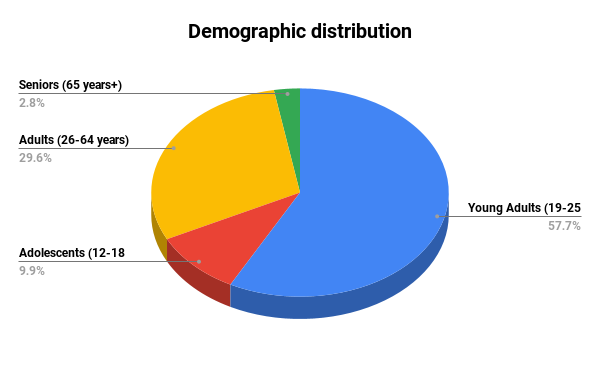
\includegraphics[width=0.75\linewidth]{Demographic-distribution.png}
                \caption{Demographic Distribution}
                \label{fig:demographic-distribution}
            \end{figure}
            \item \textbf{Travel Frequency}: Most respondents travel once every 6 months or once a year, highlighting a preference for occasional travel due to work and life commitments.
            \begin{figure}
                \centering
                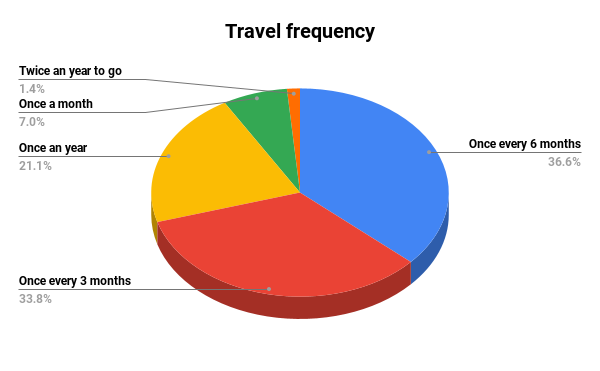
\includegraphics[width=0.75\linewidth]{Travel-frequency.png}
                \caption{Travel Frequency}
                \label{fig:travel-frequency}
            \end{figure}
            \item \textbf{Types of Travel}: Casual, entertainment, and work travel were the most common, underscoring the importance of leisure and professional commitments in travel plans.
            \begin{figure}
                \centering
                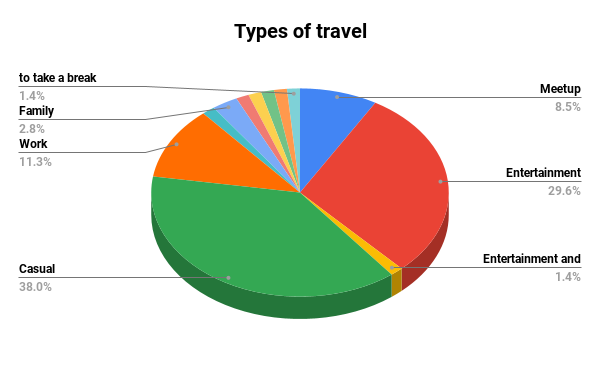
\includegraphics[width=0.75\linewidth]{Types-of-travel.png}
                \caption{Types of Travel}
                \label{fig:types-of-travel}
            \end{figure}
            \item \textbf{Itinerary Planning}: Online travel websites and YouTube videos are the primary sources for itinerary planning, showing a shift towards digital platforms and social media for travel information.
            \begin{figure}
                \centering
                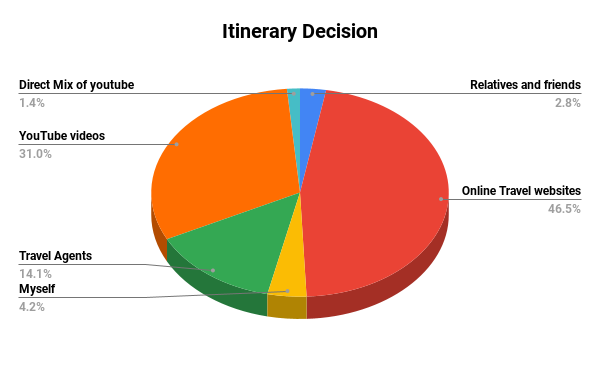
\includegraphics[width=0.75\linewidth]{Itinerary-Decision.png}
                \caption{Itinerary Decision}
                \label{fig:itenary-decision}
            \end{figure}
            \item \textbf{Customization Preferences}: A significant majority prefer customized itineraries over preselected packages, emphasizing the need for personalized travel planning tools.
            \begin{figure}
                \centering
                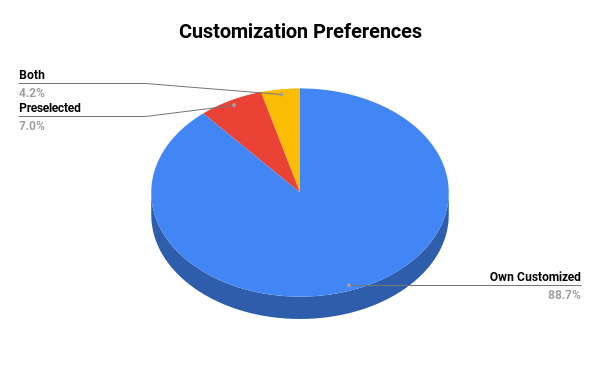
\includegraphics[width=0.75\linewidth]{Customization-Preferences.png}
                \caption{Customization Preferences}
                \label{fig:customization-preferences}
            \end{figure}
            \item \textbf{Satisfaction with Travel Agencies}: Satisfaction levels with travel agencies vary, with many users expressing moderate satisfaction, indicating potential areas for improvement in travel agency services.
            \begin{figure}
                \centering
                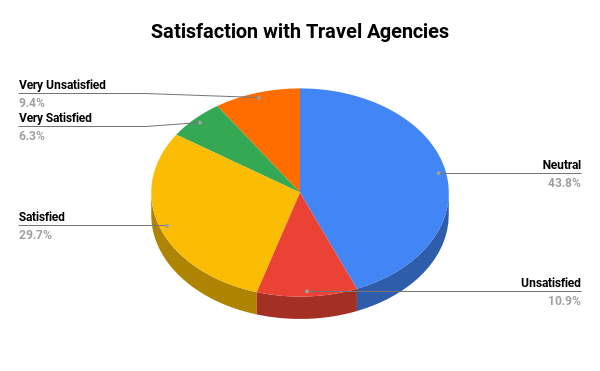
\includegraphics[width=0.75\linewidth]{Satisfaction-with-Travel-Agencies.png}
                \caption{Satisfaction with Travel Agencies}
                \label{fig:satisfaction-with-travel-agencies}
            \end{figure}
            \item \textbf{Challenges in Planning}: The main challenges include the overwhelming amount of information, coordination difficulties, and lack of personalized recommendations, making travel planning a time-consuming and stressful process.
        \end{itemize}
            \begin{figure}
                \centering
                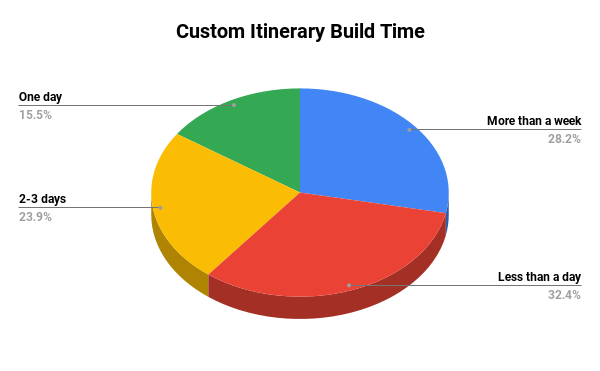
\includegraphics[width=0.75\linewidth]{Custom-Itinerary-Build-Time.png}
                \caption{Custom Itinerary Build Time}
                \label{fig:custom-itinerary-build-time}
            \end{figure}
            \begin{figure}
                \centering
                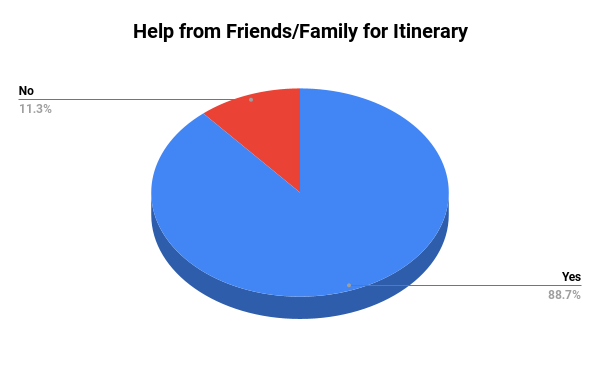
\includegraphics[width=0.75\linewidth]{Help-from-Friends-Family-for-Itinerary.png}
                \caption{Help from Friends & Family for Itinerary}
                \label{fig:help-from-friends-family-for-itinerary}
            \end{figure}

    \subsection{Interview Methodology and Findings}
        In addition to the survey, we conducted in-depth interviews with selected participants to gain deeper insights into their travel planning experiences. The interviews focused on understanding the specific pain points and expectations from a travel planning tool.
        \\

        \textbf{Key Insights from Interviews:}

        \begin{itemize}
            \item \textbf{Frequency of Travel}: Interviewees typically travel 3-4 times a year, with a mix of long vacations and short trips, emphasizing the need for flexible and comprehensive planning tools.
            \item \textbf{Planning Process}: The typical process involves extensive research using multiple online sources, comparison of prices, and seeking recommendations from friends and family, highlighting the complexity and time-consuming nature of travel planning.
            \item \textbf{Challenges}: Common challenges include dealing with an overwhelming amount of information, coordinating different trip elements, and finding reliable, personalized recommendations. These issues often lead to stress and inefficiencies in planning.
            \item \textbf{Expectations from AI Tools}: Participants expressed a strong preference for AI tools that provide tailored recommendations, streamline the booking process, and offer real-time updates. The ability to integrate multiple information sources and provide a cohesive planning experience was deemed essential.
            \item \textbf{Personalization}: The importance of personalization was reiterated, with users seeking tools that can adapt to their unique interests and preferences, ensuring a more enjoyable and relevant travel experience.
            \item \textbf{User Experience}: There is a high demand for user-friendly interfaces that offer seamless integration with other platforms, clear information presentation, and robust customer support.
        \end{itemize}

    \subsection{Ongoing Implications}
        The survey and interview findings underscore the need for a comprehensive, personalized travel planning tool like Roamify. Users face significant challenges in planning their trips, including information overload, coordination difficulties, and lack of personalized recommendations. By leveraging AI to provide tailored itineraries, real-time updates, and an intuitive user interface, Roamify can address these pain points and enhance the overall travel planning experience. The insights gained from this research will inform the development of Roamify, ensuring it meets the needs and expectations of modern travelers.


\section*{Acknowledgment}
    The authors would like to extend their sincerest gratitude to \href{https://www.iiitd.ac.in/dhruv}{Dr Dhruv Kumar} \textit{(Computer Science \& Engineering Dept., \href{https://www.iiitd.ac.in/}{IIIT-Delhi})} for their invaluable guidance throughout the project. Their insightful feedback and expertise have been instrumental in shaping this project into its final form.


\newpage

\begin{thebibliography}{1}

    \bibitem{IEEEhowto:kopka}
        @article{article,
        author = {Filho, Angelo and Morabito, Reinaldo},
        year = {2023},
        month = {11},
        pages = {122437},
        title = {An effective approach for bi-objective multi-period touristic itinerary planning},
        volume = {240},
        journal = {Expert Systems with Applications},
        doi = {10.1016/j.eswa.2023.122437}
        }
    
    \bibitem{IEEEhowto:openai}
        OpenAI. (2023). "ChatGPT Release Notes." Retrieved from \url{https://help.openai.com/en/articles/6825453-chatgpt-release-notes}.
    
    \bibitem{IEEEhowto:econsultancy}
        Econsultancy. (2023). "Travel: How OTAs are adding generative AI to test the future of trip planning." Retrieved from \url{https://econsultancy.com/travel-ota-generative-ai/}.
    
    \bibitem{IEEEhowto:srdvtechnologies}
        SRDV Technologies. (2023). "Major Challenges Faced by Online Travel Agencies." Retrieved from \url{https://www.srdvtechnologies.com/blog/major-challenges-faced-by-online-travel-agencies}.
    
    \bibitem{ip2location}
        IP2Location, \emph{IP2Location IATA ICAO CSV}, \href{https://github.com/ip2location/ip2location-iata-icao/blob/master/iata-icao.csv}{https://github.com/ip2location/ip2location-iata-icao/blob/master/iata-icao.csv}.
    
    \bibitem{transformers}
        Hugging Face, \emph{Transformers Issue 27985 (with tracking parameters)}, \href{https://github.com/huggingface/transformers/issues/27985}{https://github.com/huggingface/transformers/issues/27985}.
    
    \bibitem{stackoverflow}
        Stack Overflow. Retrieved from \url{https://stackoverflow.com}.
    
    \bibitem{metawebsite}
        Meta. Retrieved from \url{https://about.meta.com}.
    
    \bibitem{youtube}
        YouTube, \emph{For training Llama Model using QLora and PEfT}, \href{https://www.youtube.com/watch?v=Vg3dS-NLUT4}{https://www.youtube.com/watch?v=Vg3dS-NLUT4}.
    
    \bibitem{llama}
        GitHub, \emph{Llama GitHub repository}, \href{https://github.com/facebookresearch/llama.git}{https://github.com/facebookresearch/llama.git}.
    
    \bibitem{spaCy}
        Explosion. (2023). "spaCy: Industrial-strength Natural Language Processing in Python." Retrieved from \url{https://spacy.io}.
    
    \bibitem{t5paper}
        Raffel, Colin, et al. "Exploring the limits of transfer learning with a unified text-to-text transformer." \emph{Journal of Machine Learning Research} 21.140 (2020): 1-67.
    
    \bibitem{bertpaper}
        Devlin, Jacob, et al. "BERT: Pre-training of Deep Bidirectional Transformers for Language Understanding." \emph{arXiv preprint arXiv:1810.04805} (2018).
    
    \bibitem{roberapaper}
        Liu, Yinhan, et al. "RoBERTa: A Robustly Optimized BERT Pretraining Approach." \emph{arXiv preprint arXiv:1907.11692} (2019).
    
    \bibitem{distilbertpaper}
        Sanh, Victor, et al. "DistilBERT, a distilled version of BERT: smaller, faster, cheaper and lighter." \emph{arXiv preprint arXiv:1910.01108} (2019).
    
    \bibitem{llamapaper}
        Touvron, Hugo, et al. "LLaMA: Open and Efficient Foundation Language Models." \emph{arXiv preprint arXiv:2302.13971} (2023).
    
    \bibitem{huggingface}
        Hugging Face. (2023). "Transformers: State-of-the-art Machine Learning for Pytorch, TensorFlow, and JAX." Retrieved from \url{https://github.com/huggingface/transformers}.
    
    \bibitem{nltk}
        Bird, Steven, Edward Loper, and Ewan Klein. "Natural language processing with Python: analyzing text with the natural language toolkit." \emph{"O'Reilly Media, Inc."} (2009).
    
    \bibitem{unsloth}
        Unsloth, \emph{Unsloth: An Efficient Library for Training Large Language Models}, \href{https://github.com/unsloth/unsloth}{https://github.com/unsloth/unsloth}.
    
    \bibitem{webscraping}
        Mitrevski, Marko. "Python Web Scraping: Hands-On Data Scraping and Crawling Using Pyspider, Splash, and Selenium." \emph{"Packt Publishing Ltd."} (2020).
    
    \bibitem{pythonselenium}
        SeleniumHQ. (2023). "Selenium WebDriver." Retrieved from \url{https://www.selenium.dev}.
    
    \bibitem{flant5}
        Heidloff, Niklas. (2023). "Fine-Tuning FLAN-T5." Retrieved from \url{https://heidloff.net/article/fine-tuning-flan-t5/}.
    
    \bibitem{flant5dc}
        DataCamp. (2023). "FLAN-T5 Tutorial." Retrieved from \url{https://www.datacamp.com/tutorial/flan-t5-tutorial}.
    
    \bibitem{flant5yt}
        YouTube. (2023). "FLAN-T5 Tutorial." Retrieved from \url{https://www.youtube.com/watch?v=PyRbP9d27sk}.
    
    \bibitem{llama3a}
        GitHub. (2023). "Unsloth: Efficient Library for Training Large Language Models." Retrieved from \url{https://github.com/unslothai/unsloth}.
    
    \bibitem{llama3b}
        Hugging Face Blog. (2023). "Fine-Tuning LLaMA-3 with Unsloth." Retrieved from \url{https://huggingface.co/blog/mlabonne/sft-llama3}.
    
    \bibitem{simpletransformers1}
        Towards Data Science. (2023). "Simple Transformers: Introducing the Easiest BERT, RoBERTa, XLNet, and XLM Library." Retrieved from \url{https://towardsdatascience.com/simple-transformers-introducing-the-easiest-bert-roberta}.
        % https://towardsdatascience.com/simple-transformers-introducing-the-easiest-bert-roberta-xlnet-and-xlm-library-58bf8c59b2a3
    
    \bibitem{simpletransformers2}
        YouTube. (2023). "Simple Transformers Tutorial." Retrieved from \url{https://www.youtube.com/watch?v=3XiJrn_8F9Q&t=1058s}.

\end{thebibliography}

\newpage

\appendix

\section{User Survey}
    To understand the travel planning behaviors and preferences of potential users for Roamify, we conducted a comprehensive survey. Below are the survey questions and the options provided for multiple-choice questions.
    \\

    \begin{enumerate}
        \item \textbf{What is your name?}

        \item \textbf{Which age group do you belong to?}
        \begin{itemize}
            \item Middle Childhood (6-11 years)
            \item Adolescents (12-18 years)
            \item Young Adults (19-25 years)
            \item Adults (26-64 years)
            \item Seniors (65 years+)
        \end{itemize}

        \item \textbf{How frequently do you travel?}
        \begin{itemize}
            \item Once a month
            \item Once every 3 months
            \item Once every 6 months
            \item Once a year
            \item Other
        \end{itemize}

        \item \textbf{What is the type of travel you usually undergo?}
        \begin{itemize}
            \item Work
            \item Entertainment
            \item Casual
            \item Meetup
            \item Other
        \end{itemize}

        \item \textbf{How do you decide your itinerary?}
        \begin{itemize}
            \item Travel Agents
            \item YouTube videos
            \item Online Travel websites
            \item Other
        \end{itemize}

        \item \textbf{Do you like to travel based on your own customized itinerary or preselected recommended tourist packages?}
        \begin{itemize}
            \item Own Customized
            \item Preselected Recommended Tourist Packages
            \item Other
        \end{itemize}

        \item \textbf{If you have used a travel agency how much are you satisfied with their itinerary?}
        \begin{itemize}
            \item 1
            \item 2
            \item 3
            \item 4
            \item 5
        \end{itemize}

        \item \textbf{If you make custom itinerary how long do you take to build one?}
        \begin{itemize}
            \item Open-ended response
        \end{itemize}

        \item \textbf{Do you ask your friends and family for help who are currently living or have visited that place?}
        \begin{itemize}
            \item Yes
            \item No
        \end{itemize}
    \end{enumerate}
    \\

\newpage

\section{Interview Questions}
\\
    In addition to the survey, we conducted in-depth interviews with selected participants to gain deeper insights into their travel planning experiences. Below are the interview questions:
    \\

    \begin{enumerate}
        \item How frequently do you travel?
        \item Can you describe your typical process for planning a trip?
        \item What challenges do you face when planning a trip online?
        \item Have you ever used an offline travel agency? How was your experience compared to planning trips online?
        \item What features would you find most helpful in a travel planning tool?
        \item How important is the personalization of travel recommendations to you?
        \item Can you provide an example of a travel planning experience that was particularly stressful or frustrating?
        \item How do you think AI can improve the travel planning experience?
        \item What do you expect from a travel planning app or tool in terms of user experience?
        \item Have you ever used an AI-driven travel planning website where you can ask for personalized travel suggestions? If so, how was your experience?
    \end{enumerate}

\end{document}
